
\section{Abordagem Exploratória}

\indent Possível é abordar de forma exploratória a análise de sistemas de software
através de dados coletados durante sua execução. O conhecimento disponível do
sistema está sujeito ao que foi executado e, portanto, explorado. A instrumenção
de software em execução se justifica pelas informações disponíveis nesse
contexto.

As informações coletadas são utilizadas para se construir um grafo onde os
vértices correspondem a trechos de código em determinado tempo e, as arestas,
relações entre eles. Tal grafo recebe o nome de grafo exploratório $G_e$ onde o
grafo exploratório de $n$ execuções é denotado por $\underset{n}{G_e}$, de modo
que:

\begin{center}
  $\underset{n}{G_e} = \bigcup\limits_{i=1}^n G_{e_i},
   \qquad i \in \{ 1,2,3,...,n \}.$
\end{center}

Um grafo exploratório, por conter informações relativas à execução de um
subconjunto de trechos de código de determinado software, possui características
temporais, onde um mesmo trecho de código pode estar representado em diferentes
vértices do grafo, cada qual registrado em um certo instante de tempo. O grafo
mapa $G_m$ --- e, de forma análoga, o grafo mapa de $n$ execuções
$\underset{n}{G_m}$ --- pode ser obitido por:

\begin{center}
  $\mathcal{M}:G_e \rightarrow G_m$,
\end{center}

onde $\mathcal{M}$ é chamada função mapeadora, composta por um processo de
seleção, classificação e descrição. As figuras \ref{Figure021-Recursion}
e \ref{Figure021-IndirectRecursion} exemplificam as diferenças entre os
grafos $G_e$ e $G_m$.

Seja $C$ um conjunto que contém $k$ classificações tal que:

\begin{center}
  $D_k \in C, \quad k \in \{ 1, 2, 3, .., c \}$,
\end{center}

função descritora $\mathcal{D}$:

\begin{center}
  $\mathcal{D}:D_k \rightarrow G, \quad G \subseteq {G_m}$,
\end{center}

\begin{center}
  $\mathcal{S}:G_e \rightarrow S_e^y$,
   \\
   \hfill \break
  $S_e^y = \bigcup\limits_{j=1}^y T_{e_j},
   \quad T_{e_j} \subseteq G_e,
   \quad j \in \{ 1, 2, 3, .., y \}$,
\end{center}

e função classificadora $\mathcal{C}$:

\begin{center}
  $\mathcal{C}:T_{e_j} \rightarrow D_k$,
\end{center}

o processo de se mapear um grafo exploratótio $G_e$ é dado por:

\begin{center}
  Se $\quad \mathcal{C}({S_e^y}) = {G_e^c},
      \quad \mathcal{D}({G_e^c}) = {G_m}$, então
      \\
      \hfill \break
     $\mathcal{M}({G_e}) = \mathcal{D}(\mathcal{C}(\mathcal{S}({G_e}))) = {G_m}$.
\end{center}

{
  \centering
  \captionsetup{type=figure}
	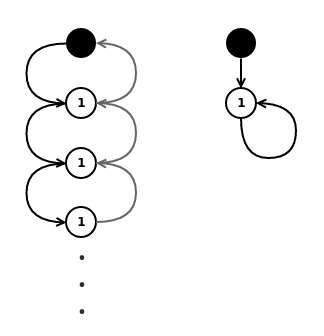
\includegraphics[scale=0.5]{./figures/Figure021-Recursion.png}
  \captionof{figure}{
    grafo exploratório (esquerda) e grafo mapa (direita) para
    recursão simples. Cada chamada a um algoritmo recursivo é representada por
    um vértice diferente no grafo exploratório, enquanto que chamadas recursivas
    são representadas por laços no grafo mapa.
    \hfill \break}
	\label{Figure021-Recursion}
}

{
  \centering
  \captionsetup{type=figure}
	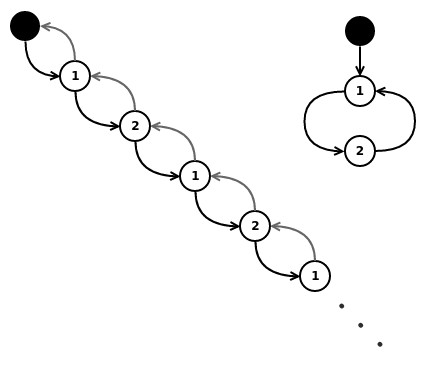
\includegraphics[width=\columnwidth]{./figures/Figure022-IndirectRecursion.png}
  \captionof{figure}{
    grafo exploratório (esquerda) e grafo mapa (direita) para
    recursão indireta. Cada chamada para trechos 1 e 2 de um algoritmo recursivo
    indireto são representadas por vértices diferentes, enquanto que o grafo
    mapa ilustra a relação de recursividade indireta entre tais trechos de forma
    concisa.
    \hfill \break}
	\label{Figure021-IndirectRecursion}
}

Os grafos $G_e$ e $G_m$ podem ser vistos como duas redes complexas distintas.
São dois modelos distintos de um mesmo software. Se aplicarmos diferentes
seleções no grafo exploratório, os grafos mapa resultantes correponderão a
diferentes escalas de análise do sistema de software sob estudo.

Os modelos elaborados apresentam potencial de trabalho, pois possibilitam
aplicar análises estatísticas, engenharia de software baseada em busca e
otimização, análise de produto, análise de qualidade e muitos outros.
Disponibilizam ainda métodos de percepção, onde os próprios modelos figuram
como artefatos de software.
